\documentclass{article}
\usepackage{graphicx}
\usepackage{amsmath}
\usepackage{cite}
\usepackage{color}
\usepackage{enumitem}
\usepackage{hyperref}
\usepackage{natbib}
\usepackage{tabularx}
\usepackage{natbib}
\usepackage{ragged2e}

\title{\textbf{"Principi di Reti Neurali"}}
\author{Alessandro Meloni GEPID}
\date{}
\begin{document}
\maketitle
\begin{abstract}
\begin{justify}
    Questo paper si soffermerà sull'analisi, la nascita, l'evoluzione delle reti neurali e i principi del loro funzionamento. Il punto focale sarà sicuramente quello di capire quanto un'intelligenza artificiale di questa portata, possa influire sul lavoro e la relativa organizzazione.In relazione a ciò, comprendere finquanto esse si possano spingere, quanta concorrenza potrebbero generare e i risvolti positivi/negativi sulla domanda di lavoro.
\end{justify}
\end{abstract}
\centering \tableofcontents
\centering \newpage
\section{Le Reti neurali}
\flushleft \subsection{Cosa sono?}
\begin{justify}
    Le reti neurali sono delle vere e proprie rappresentazioni informatiche, il quale funzionamento è paragonabile alla funzione e il comportamento che hanno i nostri neuroni biologici nel cervello.\\
    Molto probabilmente parlando di reti neurali, la maggior parte delle persone, non sa neanche che attualmente ne abbiamo tante in circolazione; e una tra le tante, che sicuramente ha acquisito una forte influenza, sia positiva che negativa, è ChatGpt.\\
    A parte questa piccola introduzione, noi chiamiamo le reti neurali in svariati modi, chi le chiama AI, chi le chiama con l'acronimo ANN (artificial neural network), oppure ancora SNN (simulated neural network).\citep{IBM2021} \\
    Indipendentemente dal nome che gli viene assegnato, le classifichiamo all'interno del mondo del Machine Learning (un linguaggio ad alta astrazione che ti da la possibilità, imparando da dei modelli attuali, di poter fare delle opportune previsioni future).\\
    A sua volta però risulta essere il perno di ulteriori algoritmi che vengono chiamati "deep learning": meccanismo algoritmico utilizzato dalle AI per modellare il funzionamento delle reti neurali, attraverso anche l'attribuzione di weights e biases; per esempio: riconoscere delle immagini, saper descrivere gli elementi chiave di un immagine, elementi di testo, suoni e via discorrendo.\citep{AWS2022}
\end{justify}


\flushleft\subsection{Quando sono state istituite?}

\centering \newpage
\section{Il funzionamento}

 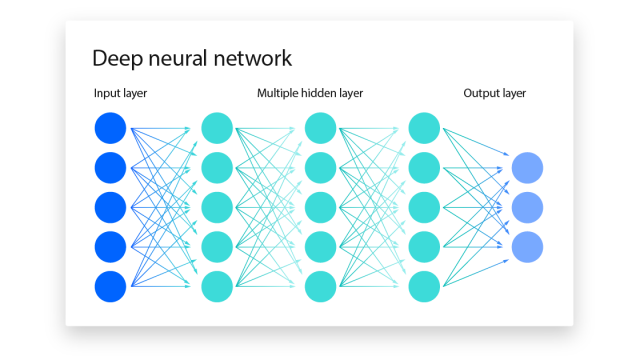
\includegraphics[width = 0.5\linewidth]{PROGETTO RETI NEURALI/ImmaginiProgetto/NeuNet.jpg}
    \label{F1:foto reti}

\flushleft \subsection{Come si comportano?}

\flushleft \subsection{A cosa servono?}
 
\flushleft \subsection{L'organizzazione e il mercato del lavoro}

\centering \newpage
\section{Considerazioni finali}
\bibliography{Database}
\bibliographystyle{alpha}
\end{document}
